This section describes the software, which was developed for the different components.
Figure \ref{software:sequence} shows the general sequence diagram of one display refresh cycle.
\begin{figure}[h]
	\centering
	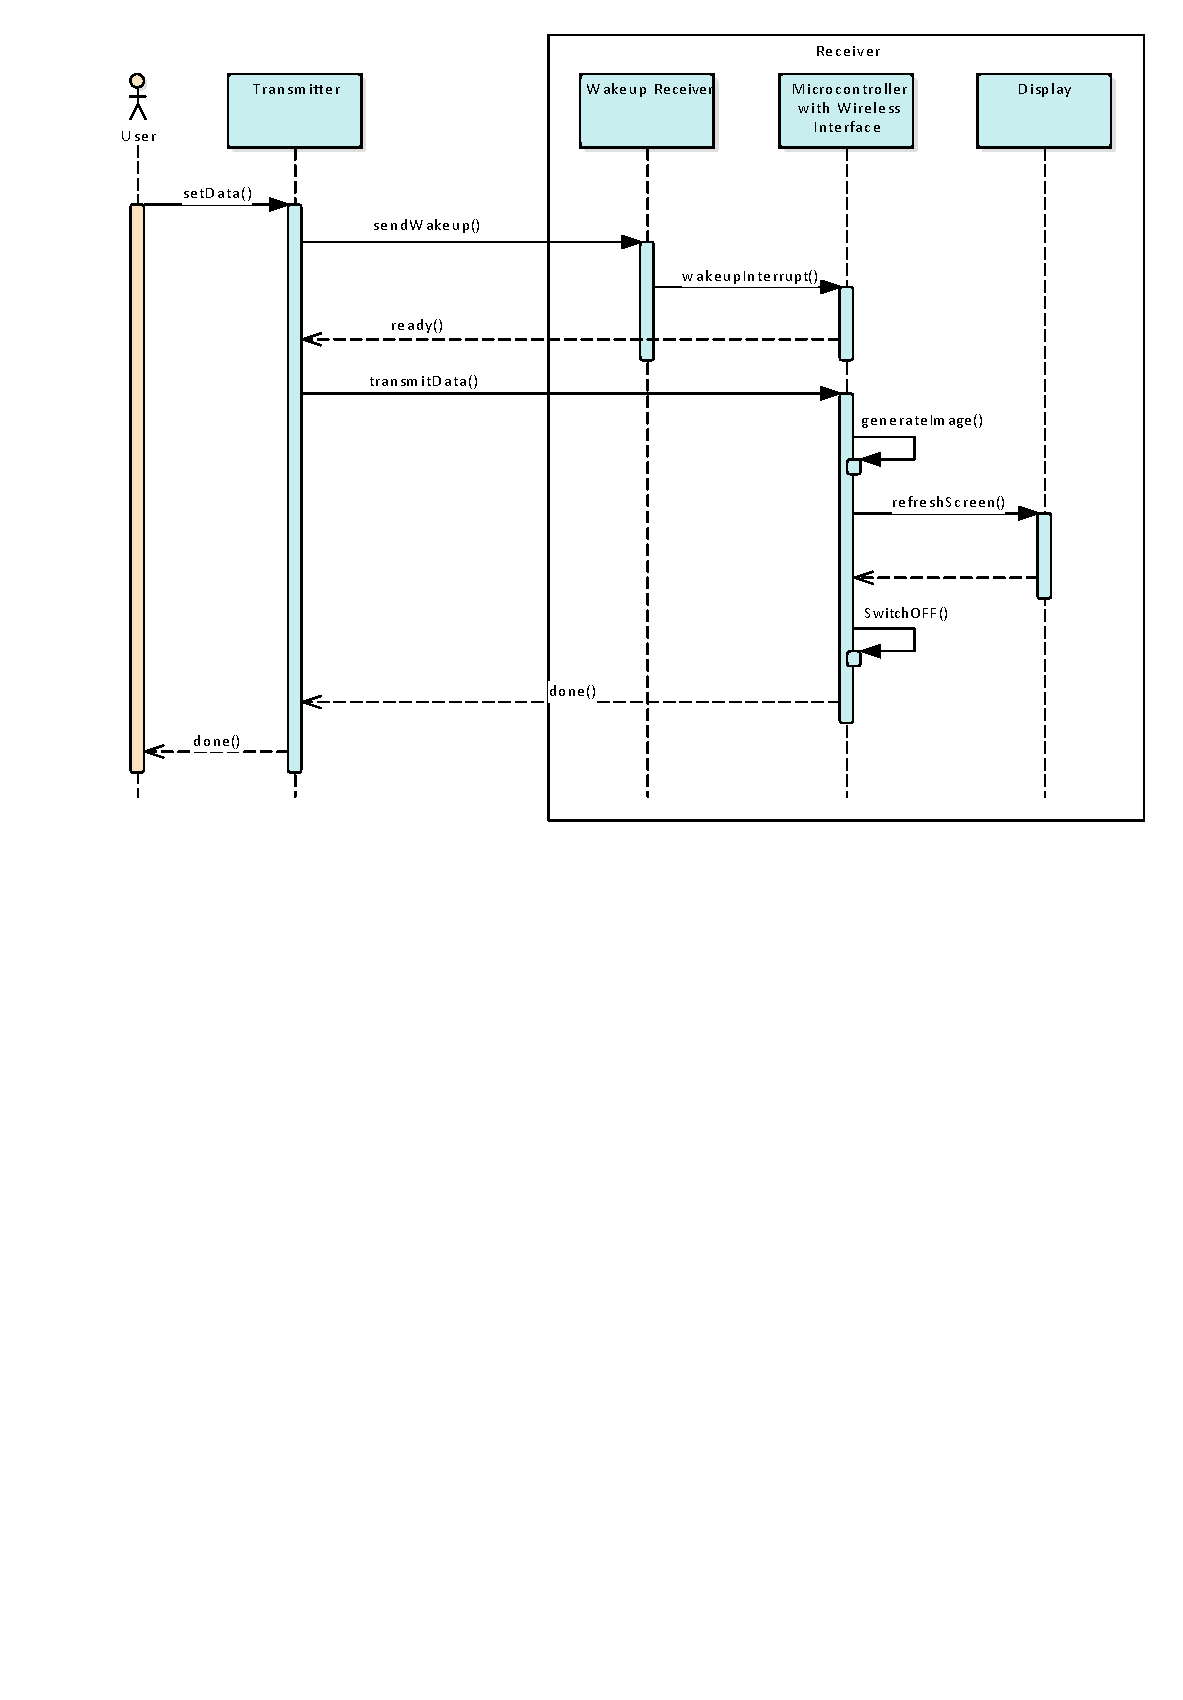
\includegraphics[width=0.9\textwidth]{4-development/software/graphics/sequence.pdf}
	\caption{Refresh sequence.\label{software:sequence}}
\end{figure}

\subsection{Receiver}
% C Style configuration
\lstdefinestyle{mystyle}{
	language=c,
	tabsize=4,
	showstringspaces=false,
	backgroundcolor = \color{gray!15!white},
	basicstyle=\scriptsize\ttfamily,
	morekeywords={as},
	keywordstyle=\color{red!80!black},
	stringstyle=\color{green!50!black},
	numberstyle=\color{red},
	emph={int,char,double,float, uint8_t, uint16_t},
	emphstyle=\color{green!50!black}
}
\lstset{style=mystyle}

\subsubsection{Microcontroller}
To develop firmware for the STM32, the Hardware abstractions layer provided by STMicroelectronics is used. The firmware running on the microcontroller is responsible for the following tasks:
\begin{itemize}[ht]
	\item[-] Initialize the IT8951 display driver chip
	\item[-] Receive data via UART from the \acs{ble}-module
	\item[-] Generate the displayed image data from a template
	\item[-] Write received text strings to the \acs{epd}
	\item[-] Write the image data to the display driver via \acs{spi}
	\item[-] Control the power supply of all the different components
\end{itemize}

\paragraph{Configurations}
The STM32 uses two bus interfaces and some extra \acs{gpio}'s to communicate and control the \acs{epd}, nRF52480 and power supply. All used pins in these interfaces are listed in Table \ref{table:stm32}.  

\begin{table}[ht]
	\begin{tabular}{ |c|c|c|c|c|c| } 
		\hline
	Description & Function &Pin number & Speed& Properties& mode \\
		\hline
	\multirow{4}{4em}{SPI} 	& Chip select & PA0&14.0\,MBits/s &No Pull-up/-down& Output \\ 
								& Clock& PA1 & 14.0\,MBits/s&No Pull-up/-down& Push Pull \\ 
								& MISO & PA6&14.0\,MBits/s & No Pull-up/-down& Push Pull  \\ 
								& MOSI & PA7& 14.0\,MBits/s&No Pull-up/-down& Push Pull  \\ 
		\hline
	\multirow{2}{4em}{UART} & TX & PC10 & 115.2\,kBits/s & Pull-up& Push Pull   \\ 
								& RX & PC11 & 115.2\,kBits/s & Pull-up& Push Pull \\ 
	\hline
	
	\multirow{2}{4em}{Power kill} & Enable & PC3 & 112\,MHz &No Pull-up/-down& Output   \\ 
										  & Disable& PC0 & 122\,MHz &No Pull-up/-down& Output \\ 
	\hline
	
	\multirow{2}{4em}{EPD interface} & Reset & PA4 & 112\,MHz &No Pull-up/-down& Output   \\ 
									& HARDY& PA5 & 122\,MHz &No Pull-up/-down& Output \\ 
	\hline

	\end{tabular}
	\caption{Table of the STM32 pin configuration.\label{table:stm32}}
\end{table}

\begin{figure}[ht]
	\centering
	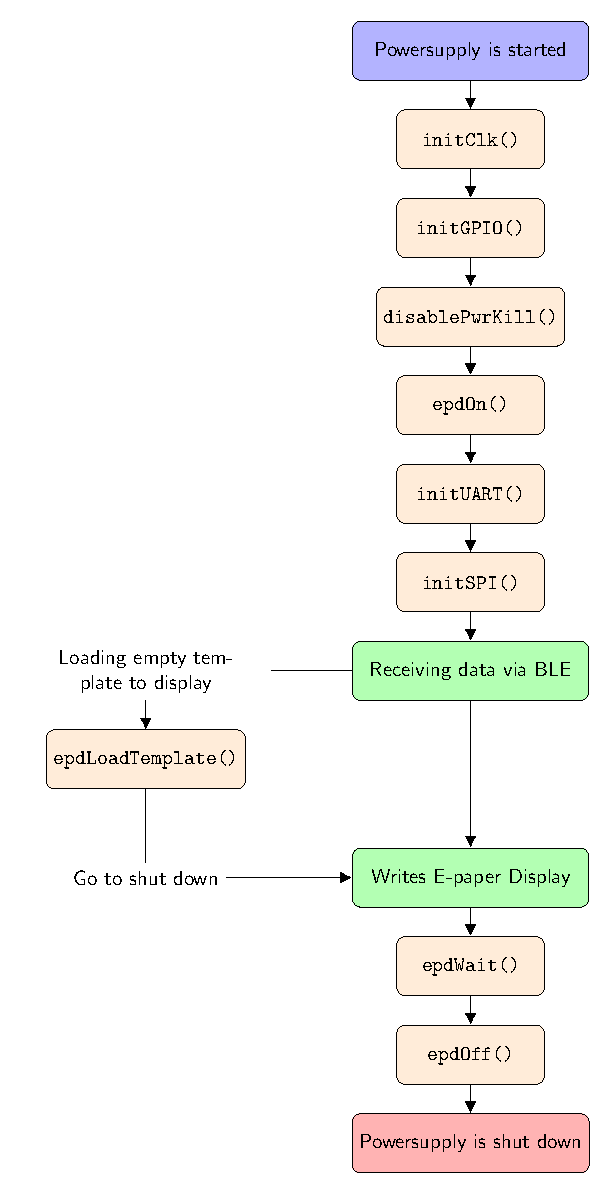
\includegraphics[height=0.8\textheight]{4-development/software/graphics/main.pdf}
	\caption{STM32 program flow chart.\label{software:main}}
\end{figure}
In the flowchart in Figure \ref{software:main} is visible, that the controller itself never enters a deep sleep mode in the end of an program cycle. Instead the controller runs trough a power kill sequence which disables it's own power supply. As a result, the controller repeats the initializing process at the begin o every wakeup.

\paragraph{IT8951 Driver}
To program the communication between the STM32 with the IT8951, a programming guide by the manufacturer ITE Tech. Inc. was used.
The interface is based on a 16-bit \acs{spi}-bus with three additional control pins. Since the IT8951 requires a big-endian format, the STM32 has to reformat all the bytes. 
The manufacturer recommends a SPI clock rate of 12\,MHz, while the maximum given in the data sheet is 24\,MHz.
This leads to a maximum transfer rate of 3\,MBytes/s  \cite{IT8951}. 
Writing an image to the \acs{epd} needs  
\begin{align}
	t_{\text{write}}=\frac{(1200\cdot 825)/2\,\text{bits}}{3\,\text{MBytes}/s}=0.165\,\text{s}.
\end{align}
Note that this calculation assumes 4 bits (for the 16 grey scales) per pixel.

The measured time for one writing cycle, including initialisation and fetching of the buffer registers, resulted in 0.168\,seconds. It is also possible to overclock the IT8951.
With 28\,MHz, it was still possible to read and write the display controller.      

\paragraph{Template}
The schedule template is preloaded to the flash of the STM32. To save memory, the file is converted into an $1200 \times 825$ PNG with the colour depth of 4 bit. The PNG then is used to create a c-file which holds an one dimensional array with all the pixel data in it. The pixel location is mapped to the memory as shown in figure\ref{theory:matrix}. 

\begin{figure}[H]
	\begin{lstlisting}
	const unsigned char schedule[]={0xff,0xff,0xff,0xff,0xff,0xff,0xff,...
									0xff,0xff,0xff,0xff,0xff,0xff,0xff,...
									.
									.
									.
									0xdd,0xdd,0xdd,0xdd,0xdd,0xdd,0xdd};
	\end{lstlisting}
\end{figure}
Each Hex number in the array resembles two pixels of each four bit. In the template shown in image\ref{software:kalender}, there are already some information given like the calendar week and weekdays. Storing the template like this uses 495000\,bits of flash memory. 
\begin{figure}[ht]
	\centering
	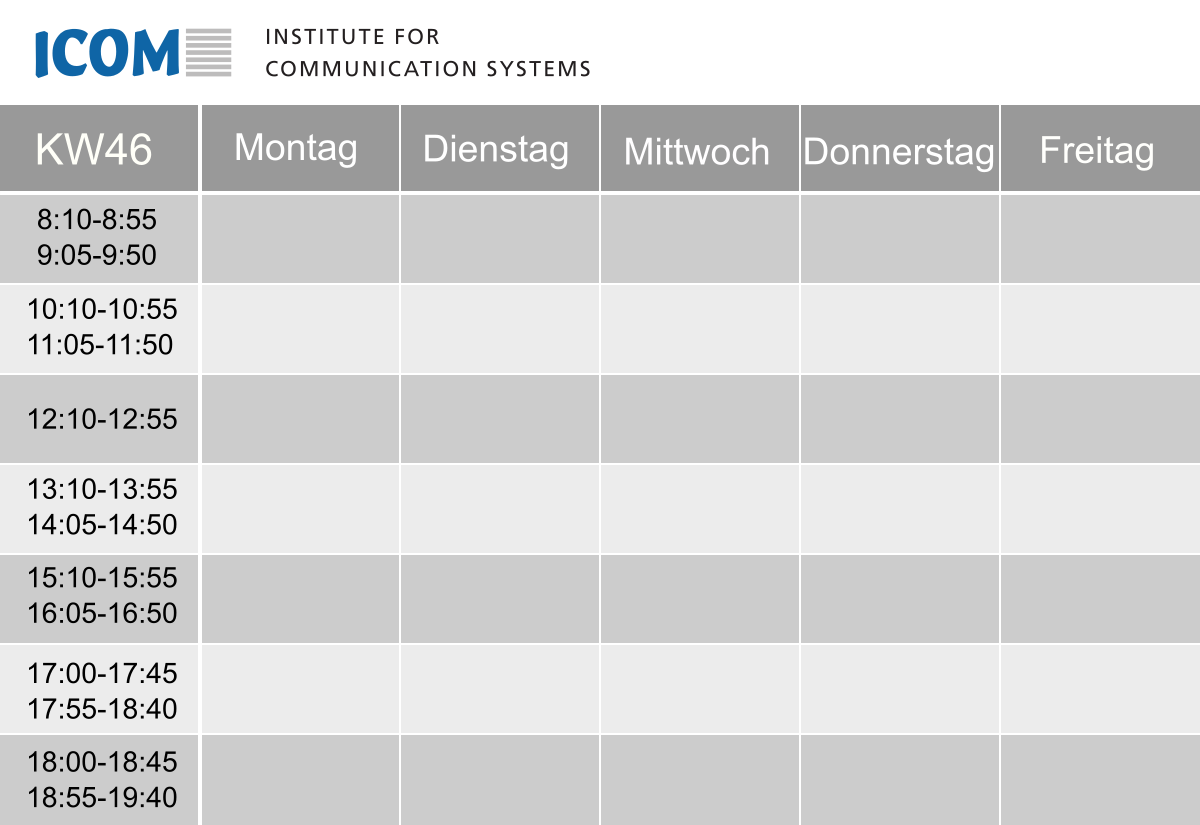
\includegraphics[height=0.6\textwidth]{4-development/software/graphics/Kalender.png}
	\caption{Example schedule used as an template.\label{software:kalender}}
\end{figure}


\paragraph{Fonts}
All fonts are c-files which hold two arrays. the first one contains all different ASCII characters, while the second array holds the font information like with and height. All characters have the compressed layout as described in Section \ref{theory:CompressedFonts}.
\begin{figure}[ht]
	\begin{lstlisting}
	const uint8_t Font12_Table[] = 
	{
		.
		.
		.,
		// @396 'A' (7 pixels wide)
		0x00, //        
		0x30, //   ##   
		0x10, //    #   
		0x28, //   # #  
		0x28, //   # #  
		0x28, //   # #  
		0x7C, //  ##### 
		0x44, //  #   # 
		0xEE, // ### ###
		0x00, //        
		0x00, //        
		0x00, // 
		.
		.
		. 
		};
		
		sFONT Font12 = {
		Font12_Table,
		7, /* Width */
		12, /* Height */
		};
	\end{lstlisting}
\end{figure}

\paragraph{Writing characters}
To write the desired characters to a image buffer, the pixel data needs to be converted and placed into the right spot. 
The code in Figure \ref{software:drawchar} shows the implemented algorithm to handle this task.
The pixel depth used in the code example is 8-bits. 
\begin{figure}[ht]
	\begin{lstlisting}
	void drawChar(uint16_t Xpt, uint16_t Ypt, const char Acsii_Char,
						sFONT* Font, uint8_t cBackground, uint8_t cForeground)
		{
			uint16_t Page, Column;
			if (Xpt > Image.Width || Ypt > Image.Height) 
			{
				return;
			}
		uint32_t Char_Offset = (Acsii_Char - ' ') * Font->Height * 
								(Font->Width / 8 + (Font->Width % 8 ? 1 : 0));
		const unsigned char *ptr = &Font->table[Char_Offset];
		
		for (Page = 0; Page < Font->Height; Page ++ ) 
		{
			for (Column = 0; Column < Font->Width; Column ++ ) 
			{
				if (FONT_BACKGROUND == cBackground) 
				{ 
					if (*ptr & (0x80 >> (Column % 8)))
						setPixel(Xpt+Column, Ypt+Page, cForeground);
				} 
				else 
				{
					if (*ptr & (0x80 >> (Column%8))) 
					{
						setPixel(Xpt + Column, Ypt + Page, cForeground);					
					} 
					else 
					{
						setPixel(Xpt + Column, Ypt + Page, cBackground);
					}
				}
				//One pixel is 8 bits
				if (Column % 8 == 7)
					ptr++;
			}
			if (Font->Width % 8 != 0)
				ptr++;
		}
	}
	\end{lstlisting}
	\caption{Write characters to image buffer.\label{software:drawchar}}
\end{figure}

All other graphical functions implemented use the \texttt{drawChar()} function to access and write information into a given display buffer. 


%\begin{figure}[ht!]
%\begin{lstlisting}
%void drawString(uint16_t xStart, uint16_t yStart,const char * pString, sFONT* Font,
%							 uint8_t cBackground,uint8_t cForeground) 
%{
%	uint16_t Ypt = yStart;
%	uint16_t Xpt = xStart;
%	
%	if (xStart > Image.Width || yStart > Image.Height)
%	{
%		return;
%	}
%	while (* pString != '\0') 
%	{
%		if ((Xpt + Font->Width ) > Image.Width ) 
%		{
%			Xpt = xStart;
%			Ypt += Font->Height;
%		}
%		if ((Ypt  + Font->Height ) > Image.Height ) 
%		{
%			Xpt = xStart;
%			Ypt = yStart;
%		}
%		drawChar(Xpt, Ypt, * pString, Font, cBackground, cForeground);
%		pString ++;
%		Xpt += Font->Width;
%	}
%}	
%\end{lstlisting}
%\end{figure}


\subsubsection{Communication}
Due to the fact that the software on both sides of the bluetooth channel is very similar it is explained in this section.
A \acs{ble} example project, which was provided by nordic, was only slightly changed to fit the purpose of this prototype.

Before a connection is established, the module on the receiver side is known as peripheral, and the module on transmitter end as the central device.
After the receiver is woken up with the RFicient, the peripheral starts advertising.
Advertising basically means sending data packets periodically with information for the central device.
The central device is scanning for the this advertisement and can decide, whether it wants to connect based on this information.
Is the connection established, it is now possible to exchange data through this channel.
This process is illustrated in Figure \ref{software:ble}.
\begin{figure}[ht]
	\centering
	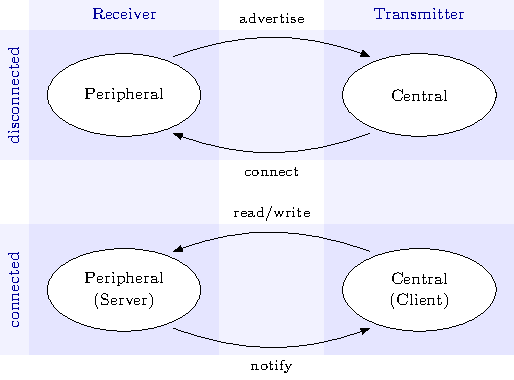
\includegraphics[width=0.8\textwidth]{4-development/software/graphics/ble.pdf}
	\caption{\acs{ble}-communication with the nRF52480.\label{software:ble}}
\end{figure}

The central device serves after connection as the client.
It can make read and write requests to access the data on the peripheral, which acts as the server.
The server on the other, hand can only send notifications to the client if new data is ready.
It should be noted, that the roles of client and server do not in any case have to be assigned to central and peripheral, but also the other way around. 

\subsection{Transmitter}

\subsubsection{Python-Script}
\lstset{basicstyle=\footnotesize}
\lstdefinestyle{mystyle}{
	language=Python,
	tabsize=4,
	showstringspaces=false,
	backgroundcolor = \color{gray!15!white},
	basicstyle=\scriptsize\ttfamily,
	morekeywords={as},
	keywordstyle=\color{blue!50!black},
	stringstyle=\color{green!50!black},
	numberstyle=\color{red},
	emph={int,char,double,float,range, len, bytes},
	emphstyle=\color{violet}
}
\lstset{style=mystyle}

A short python script enables the user to send the data to the display.
This script is presented step by step.

\begin{enumerate}
	\item Include of the used packages, time and serial.
	\begin{lstlisting}
	import serial
	import time
	\end{lstlisting}	
	\item Set desired baudrate, select which COM-port windows assigned to the development kit and open the port.
	\begin{lstlisting}
	baudrate = 115200
	com_port = 'COM14'
	
	device = serial.Serial(com_port, baudrate, writeTimeout=0)
	\end{lstlisting}
	\item Create a list of lists with the desired data.
	The first list contains information about how many packages are about to follow.
	The following list contains the location on the template, the subject and the lecturer.
	\begin{lstlisting}
	data = [[0, chr(3), '\0\0\0\0'],[11 , 'WsComm\0', 'MAH\0'],
			[3 , 'DigPro\0', 'SCU\0'], [22 , 'EmbSW\0', 'BON\0']]
	\end{lstlisting}
	\item Fill the list with \lstinline|'\0'| so every package is 20 bytes long.
	\begin{lstlisting}
	for i in range(len(data)):
		if len(data[i][1])<16:
			t = 14-len(data[i][1])
			data[i][1] = data[i][1]+'\0'*t
	\end{lstlisting}
	\item Store time when data transfer is started.
	\begin{lstlisting}
	t_start = time.time()
	\end{lstlisting}
	\item Transfer data to the nRF52480 transmitter
	\begin{lstlisting}
	for i in range(len(data)):
		device.write([data[i][0]]) 
		device.write(bytes(data[i][1], 'utf-8'))       
		device.write(bytes(data[i][2]+'\n', 'utf-8'))
		device.flush()
	\end{lstlisting}	
	\item Print elapsed time on console and close COM-port.
	\begin{lstlisting}
	print('elapsed time: {:.3f}'.format(time.time() - t_start))
	
	device.close()
	\end{lstlisting}
	
\end{enumerate}